\documentclass[facebook_diary.tex]{subfiles}

\begin{document}

\chapter{2017年}

\section{8月}

\subsection*{2017年08月05日 18:29}
\addcontentsline{toc}{subsection}{2017年08月05日 18:29}

旋盤（滝澤TSL-550）導入。

\paragraph{写真}
\begin{center}
\begin{minipage}{0.48\linewidth}
\centering
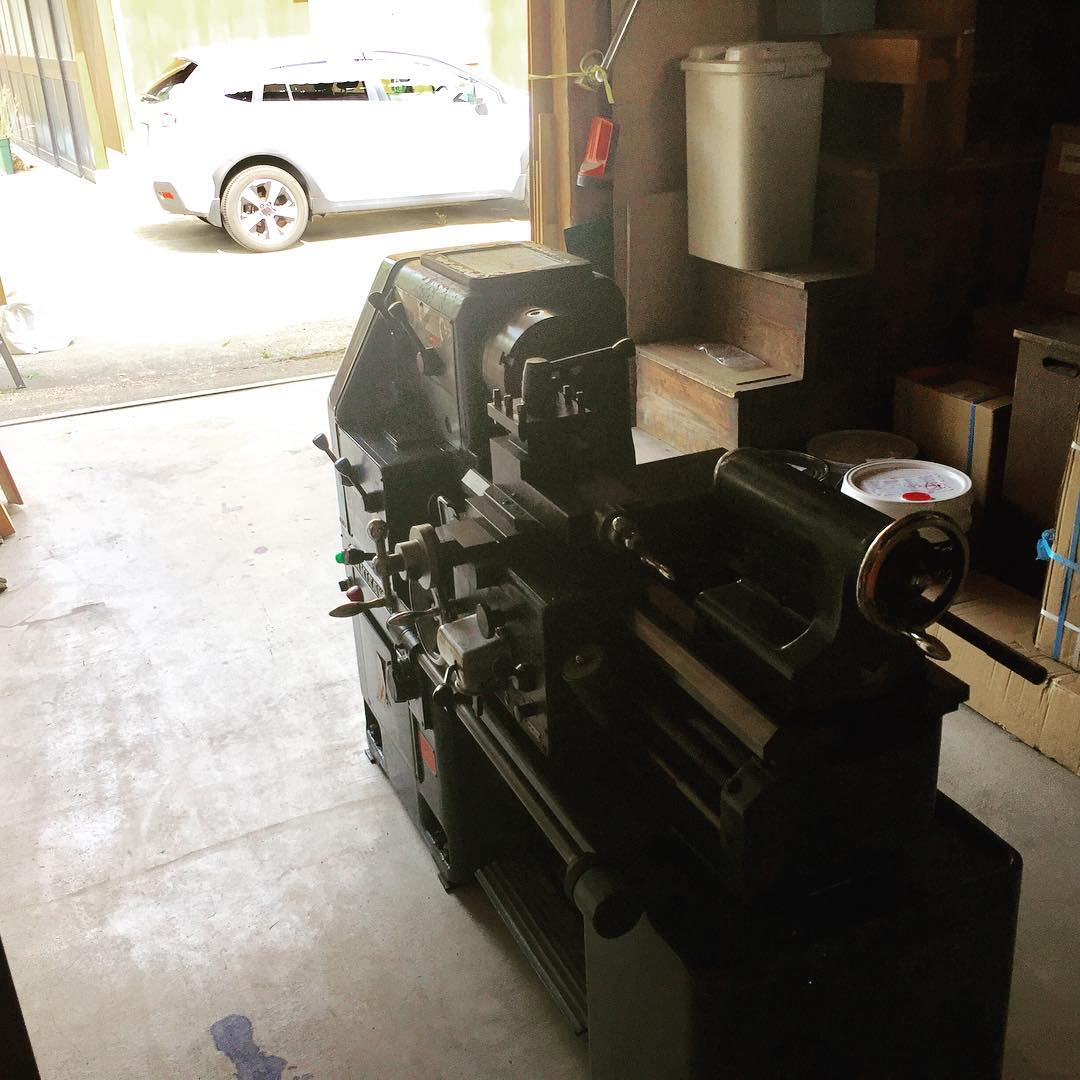
\includegraphics[width=\linewidth]{pictures/2017/08/20170805_182946_001.jpg}
\end{minipage}
\end{center}

\subsection*{2017年08月05日 18:30}
\addcontentsline{toc}{subsection}{2017年08月05日 18:30}

小さなフライス盤（井上Ⅳ-1/2）導入。

\paragraph{写真}
\begin{center}
\begin{minipage}{0.48\linewidth}
\centering
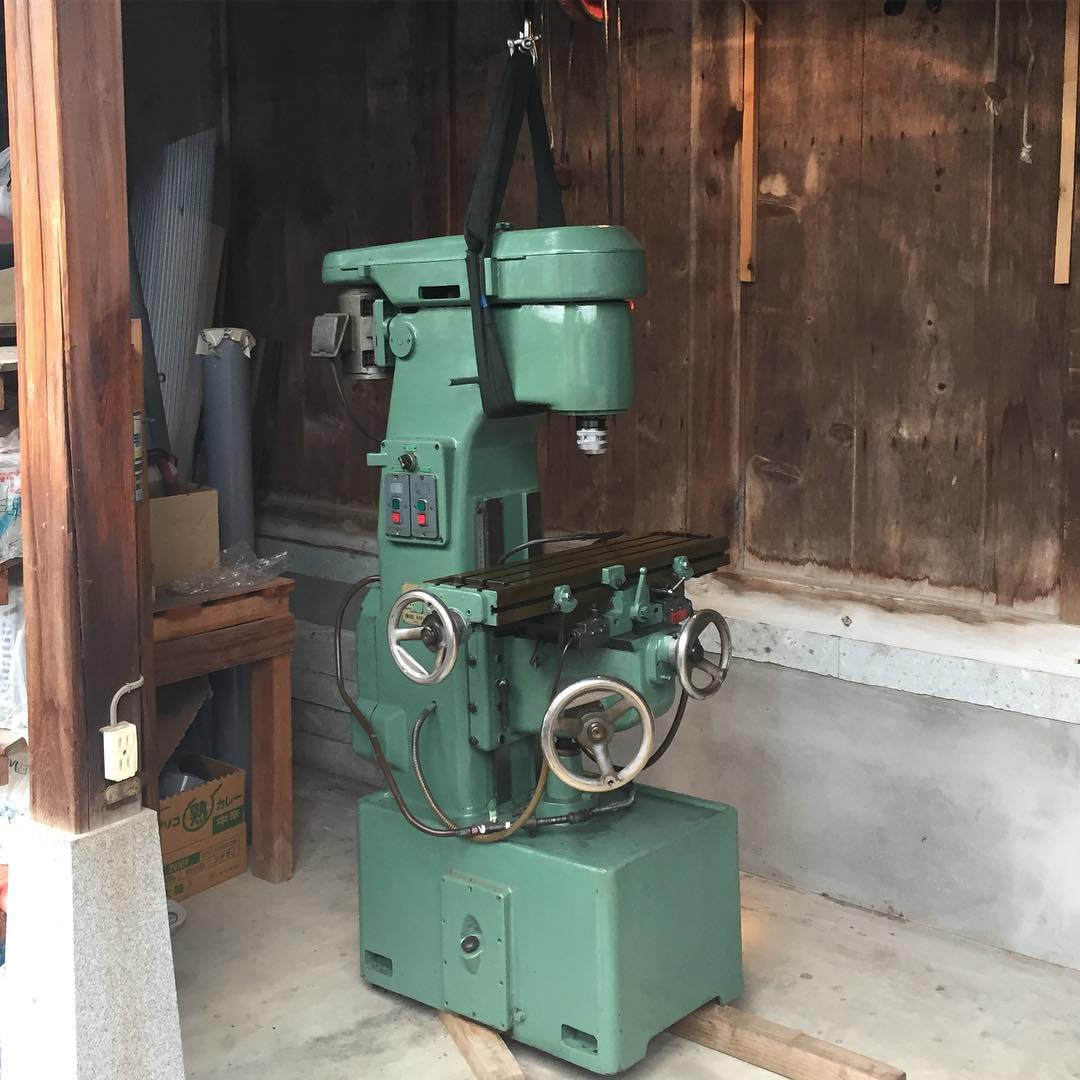
\includegraphics[width=\linewidth]{pictures/2017/08/20170805_183001_001.jpg}
\end{minipage}
\end{center}

\subsection*{2017年08月12日 23:54}
\addcontentsline{toc}{subsection}{2017年08月12日 23:54}

旋盤で段付き棒。

0.02〜0.03mmの切込み。

\paragraph{写真}
\begin{center}
\begin{minipage}{0.48\linewidth}
\centering
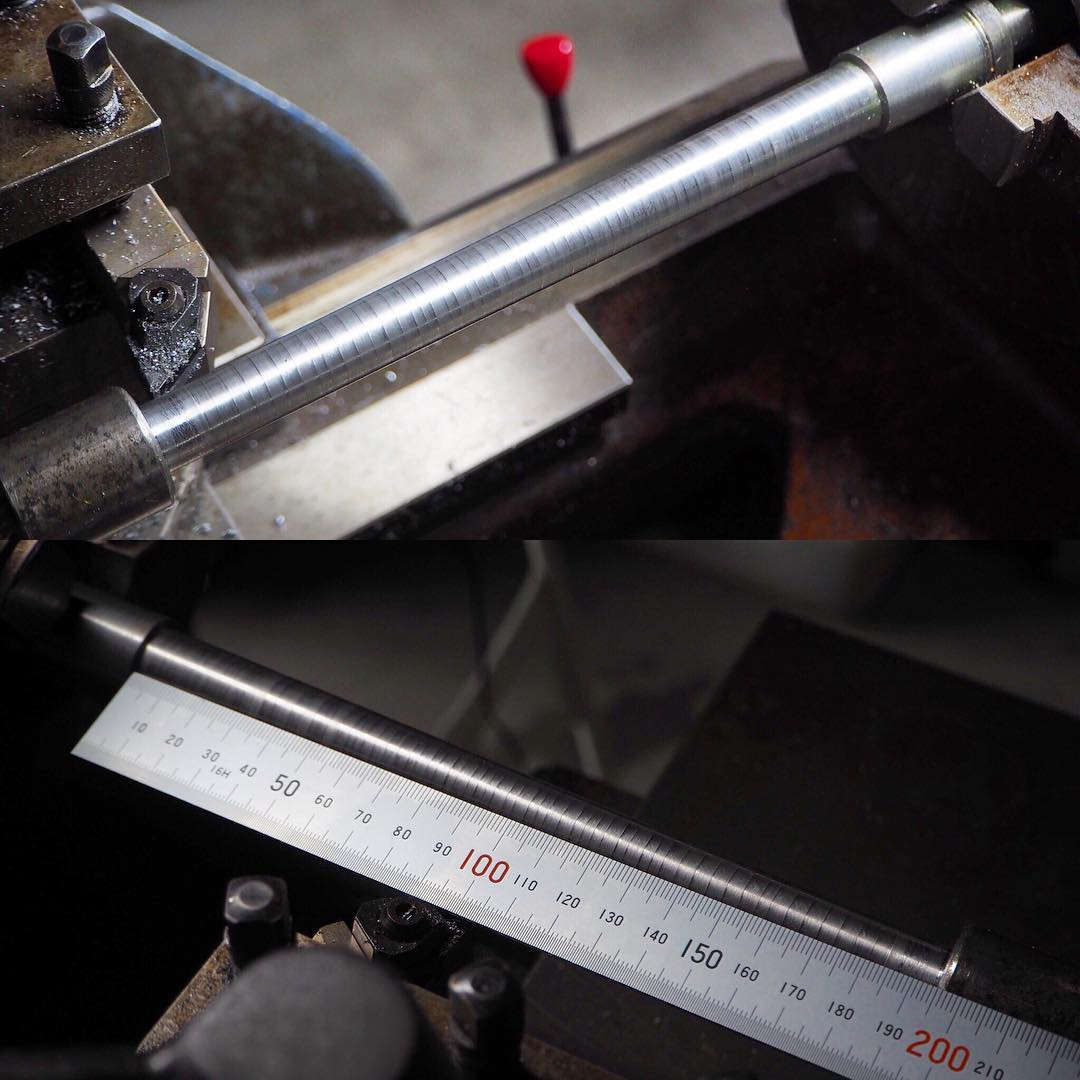
\includegraphics[width=\linewidth]{pictures/2017/08/20170812_235451_001.jpg}
\end{minipage}
\end{center}

\subsection*{2017年08月13日 00:06}
\addcontentsline{toc}{subsection}{2017年08月13日 00:06}

フライス盤にセット。Vブロックに乗せて締めると軸のセンター確定。

エンドミルは12mm。

\paragraph{写真}
\begin{center}
\begin{minipage}{0.48\linewidth}
\centering
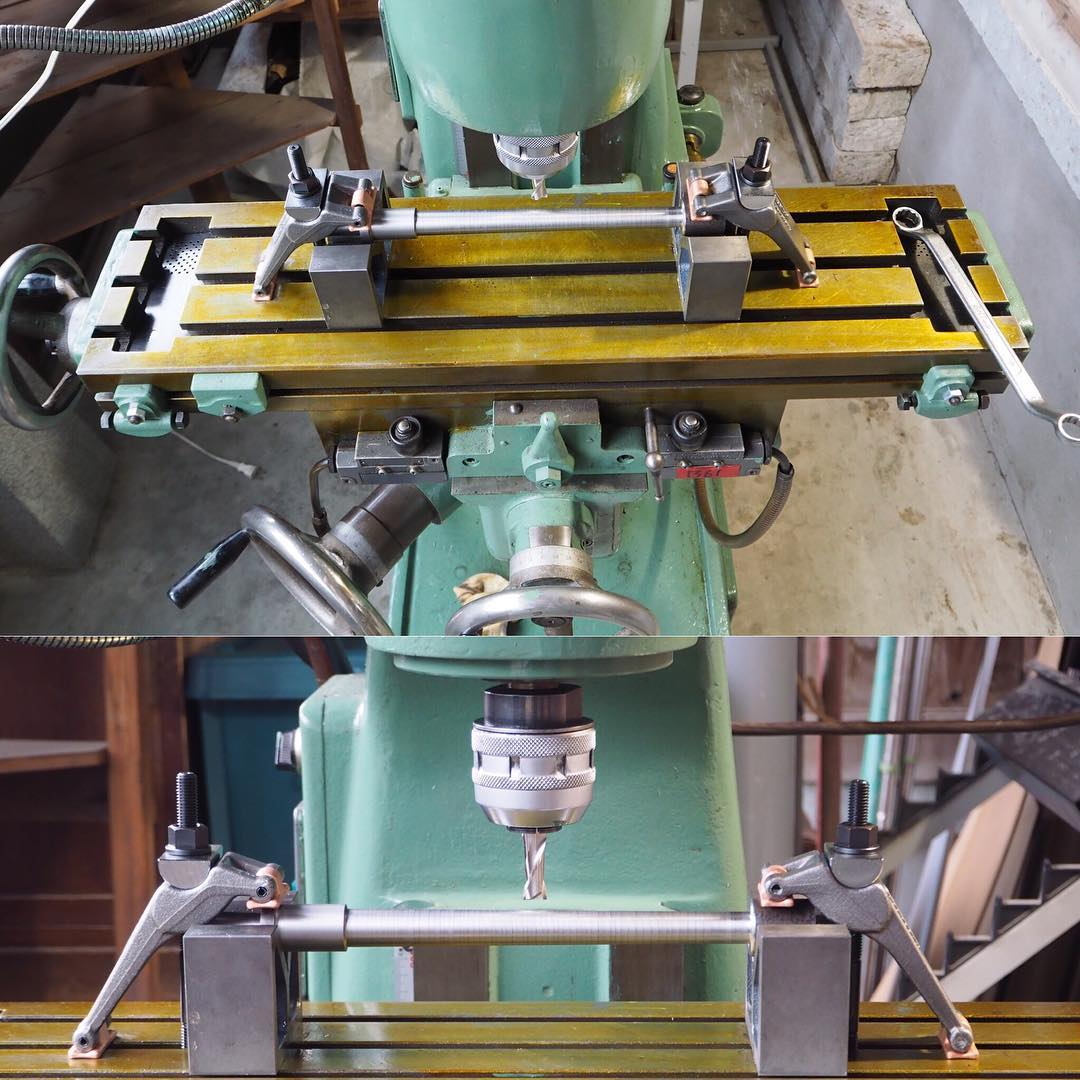
\includegraphics[width=\linewidth]{pictures/2017/08/20170813_000641_001.jpg}
\end{minipage}
\end{center}

\subsection*{2017年08月13日 00:37}
\addcontentsline{toc}{subsection}{2017年08月13日 00:37}

フライス加工開始。

\paragraph{写真}
\begin{center}
\begin{minipage}{0.48\linewidth}
\centering
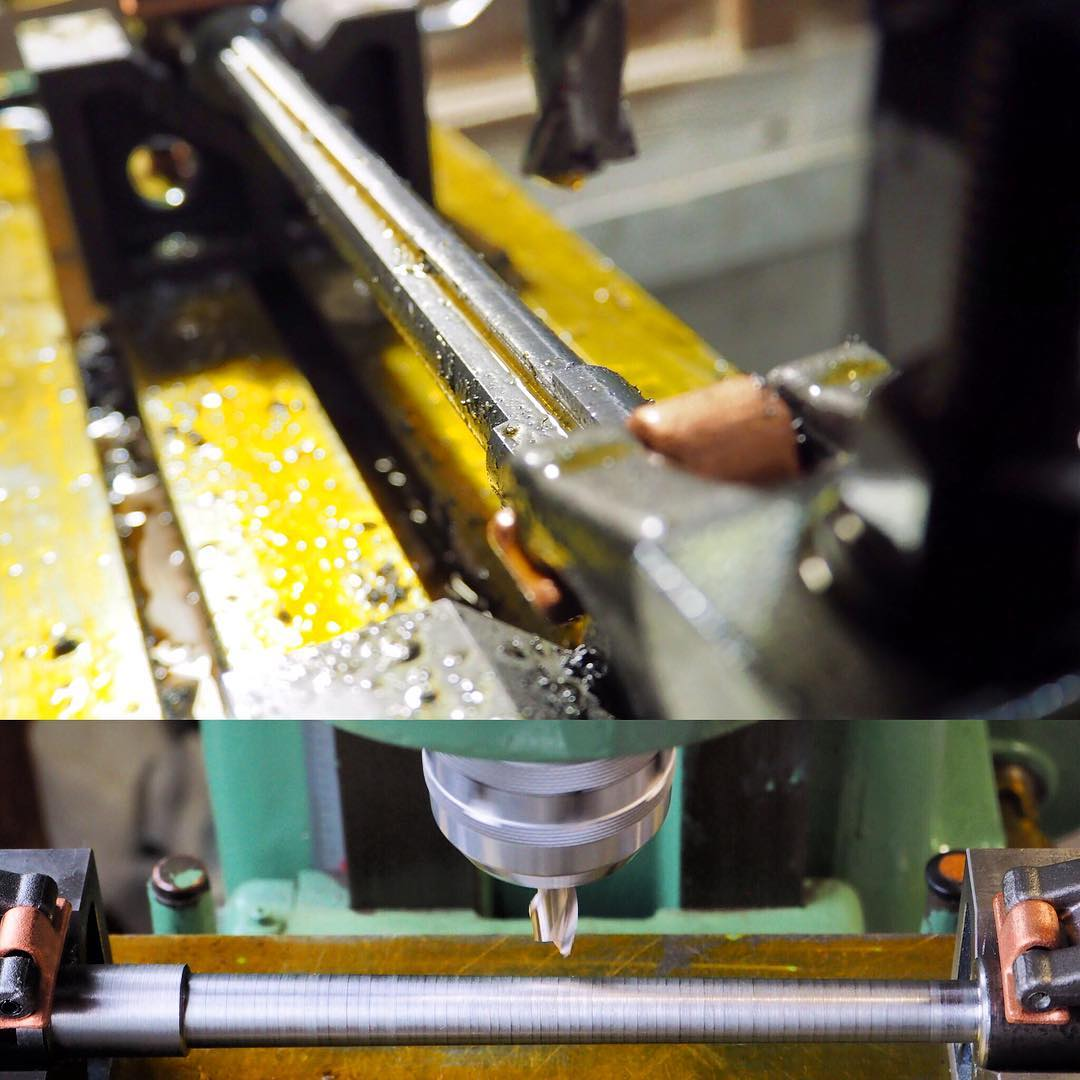
\includegraphics[width=\linewidth]{pictures/2017/08/20170813_003724_001.jpg}
\end{minipage}
\end{center}

\subsection*{2017年08月13日 08:12}
\addcontentsline{toc}{subsection}{2017年08月13日 08:12}

何ができるのでしょう？

\paragraph{写真}
\begin{center}
\begin{minipage}{0.48\linewidth}
\centering
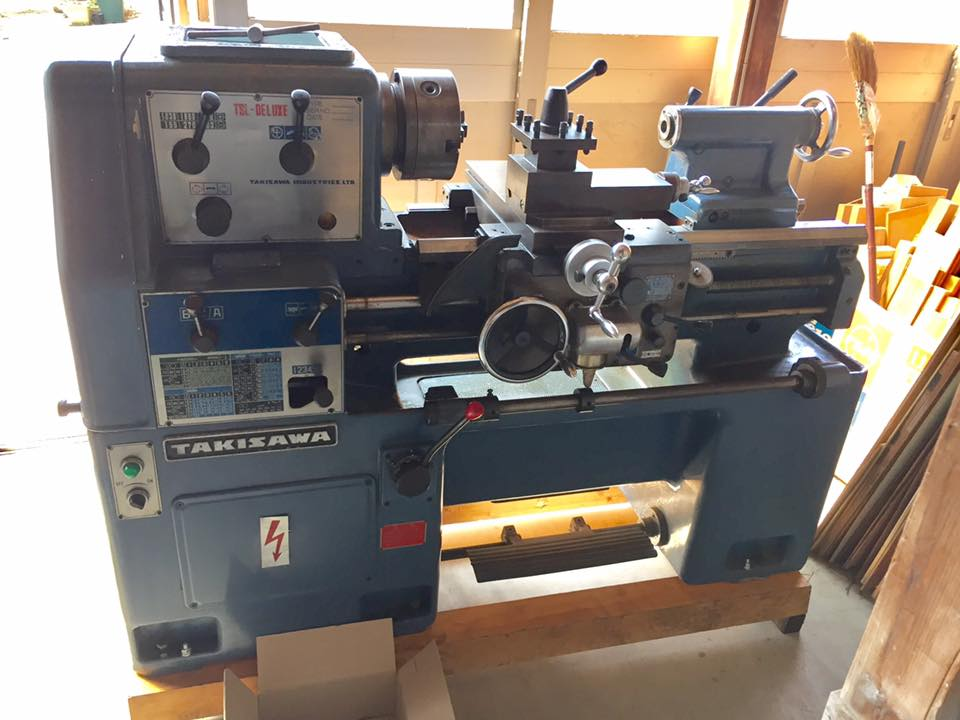
\includegraphics[width=\linewidth]{pictures/2017/08/20170813_081227_001.jpg}
\end{minipage}
\hfill
\begin{minipage}{0.48\linewidth}
\centering
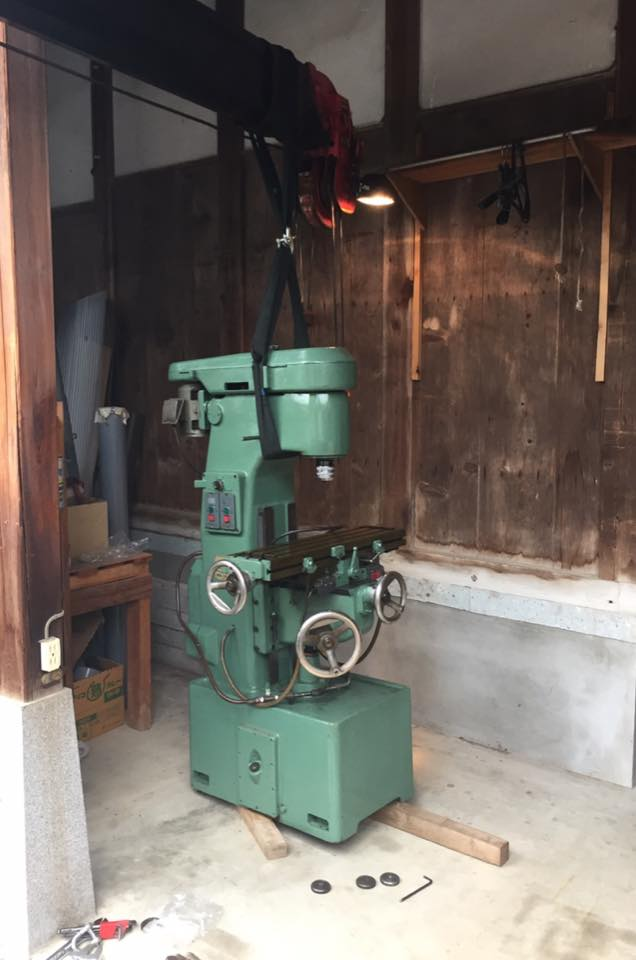
\includegraphics[width=\linewidth]{pictures/2017/08/20170813_081227_002.jpg}
\end{minipage}
\end{center}

\begin{center}
\begin{minipage}{0.48\linewidth}
\centering
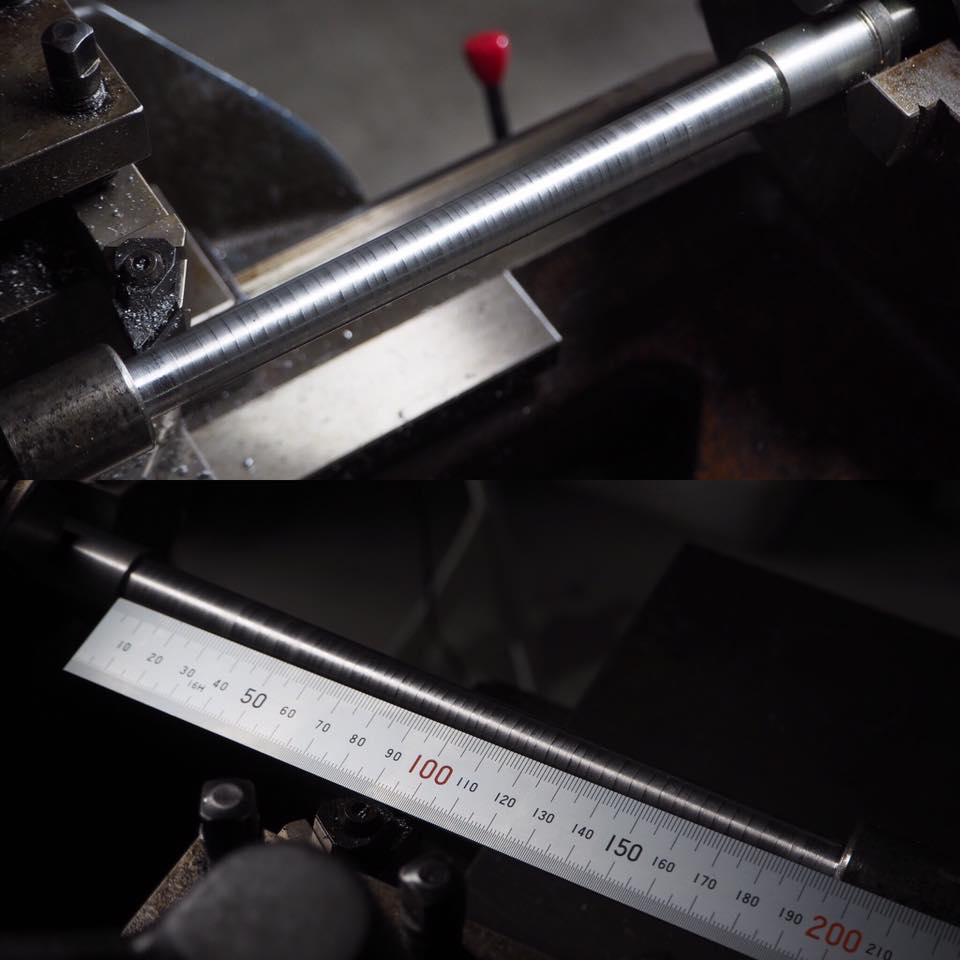
\includegraphics[width=\linewidth]{pictures/2017/08/20170813_081227_003.jpg}
\end{minipage}
\hfill
\begin{minipage}{0.48\linewidth}
\centering
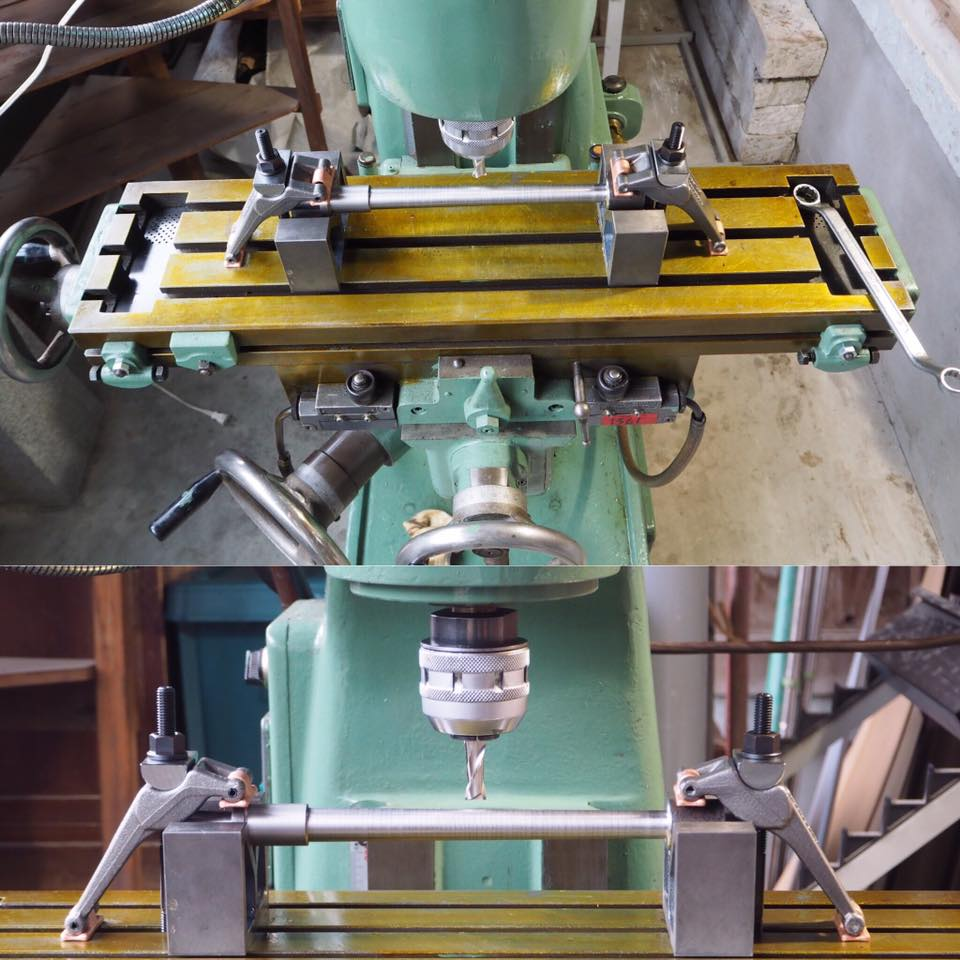
\includegraphics[width=\linewidth]{pictures/2017/08/20170813_081227_004.jpg}
\end{minipage}
\end{center}

\begin{center}
\begin{minipage}{0.48\linewidth}
\centering
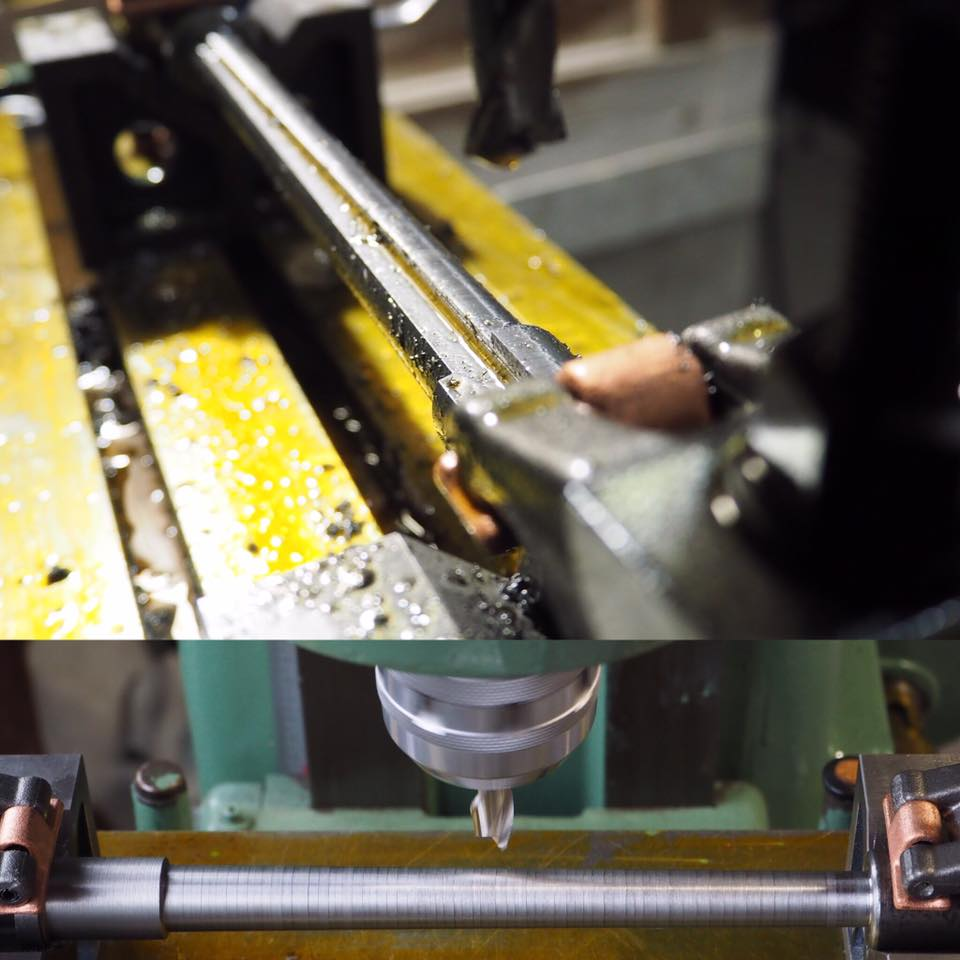
\includegraphics[width=\linewidth]{pictures/2017/08/20170813_081227_005.jpg}
\end{minipage}
\end{center}


\end{document}
